\documentclass{beamer}
\usepackage[utf8]{inputenc}
\usepackage{utopia}

\usetheme{Madrid}
\usecolortheme{default}

%------------------------------------------------------------
%This block of code defines the information to appear in the title page.
\title[Geode]
{Global analytics in the face of bandwidth and regulatory constraints}

\subtitle{Geode}

\author[Vulimiri et al., 2015]
{Ashish Vulimiri, Thomas Jungblut, Carlo Curino, Jitu Padhye, Brighten Godfrey, George Varghese}

\date[Big Data Infrastructure]
{Presented by Claudio Scheer}
%------------------------------------------------------------


%------------------------------------------------------------
\AtBeginSection[]
{
	\begin{frame}
		\frametitle{Table of Contents}
		\tableofcontents[currentsection]
	\end{frame}
}
%------------------------------------------------------------


\begin{document}

\frame{\titlepage}


\section{Methodology}
%---------------------------------------------------------
\begin{frame}
	\frametitle{Problem}
	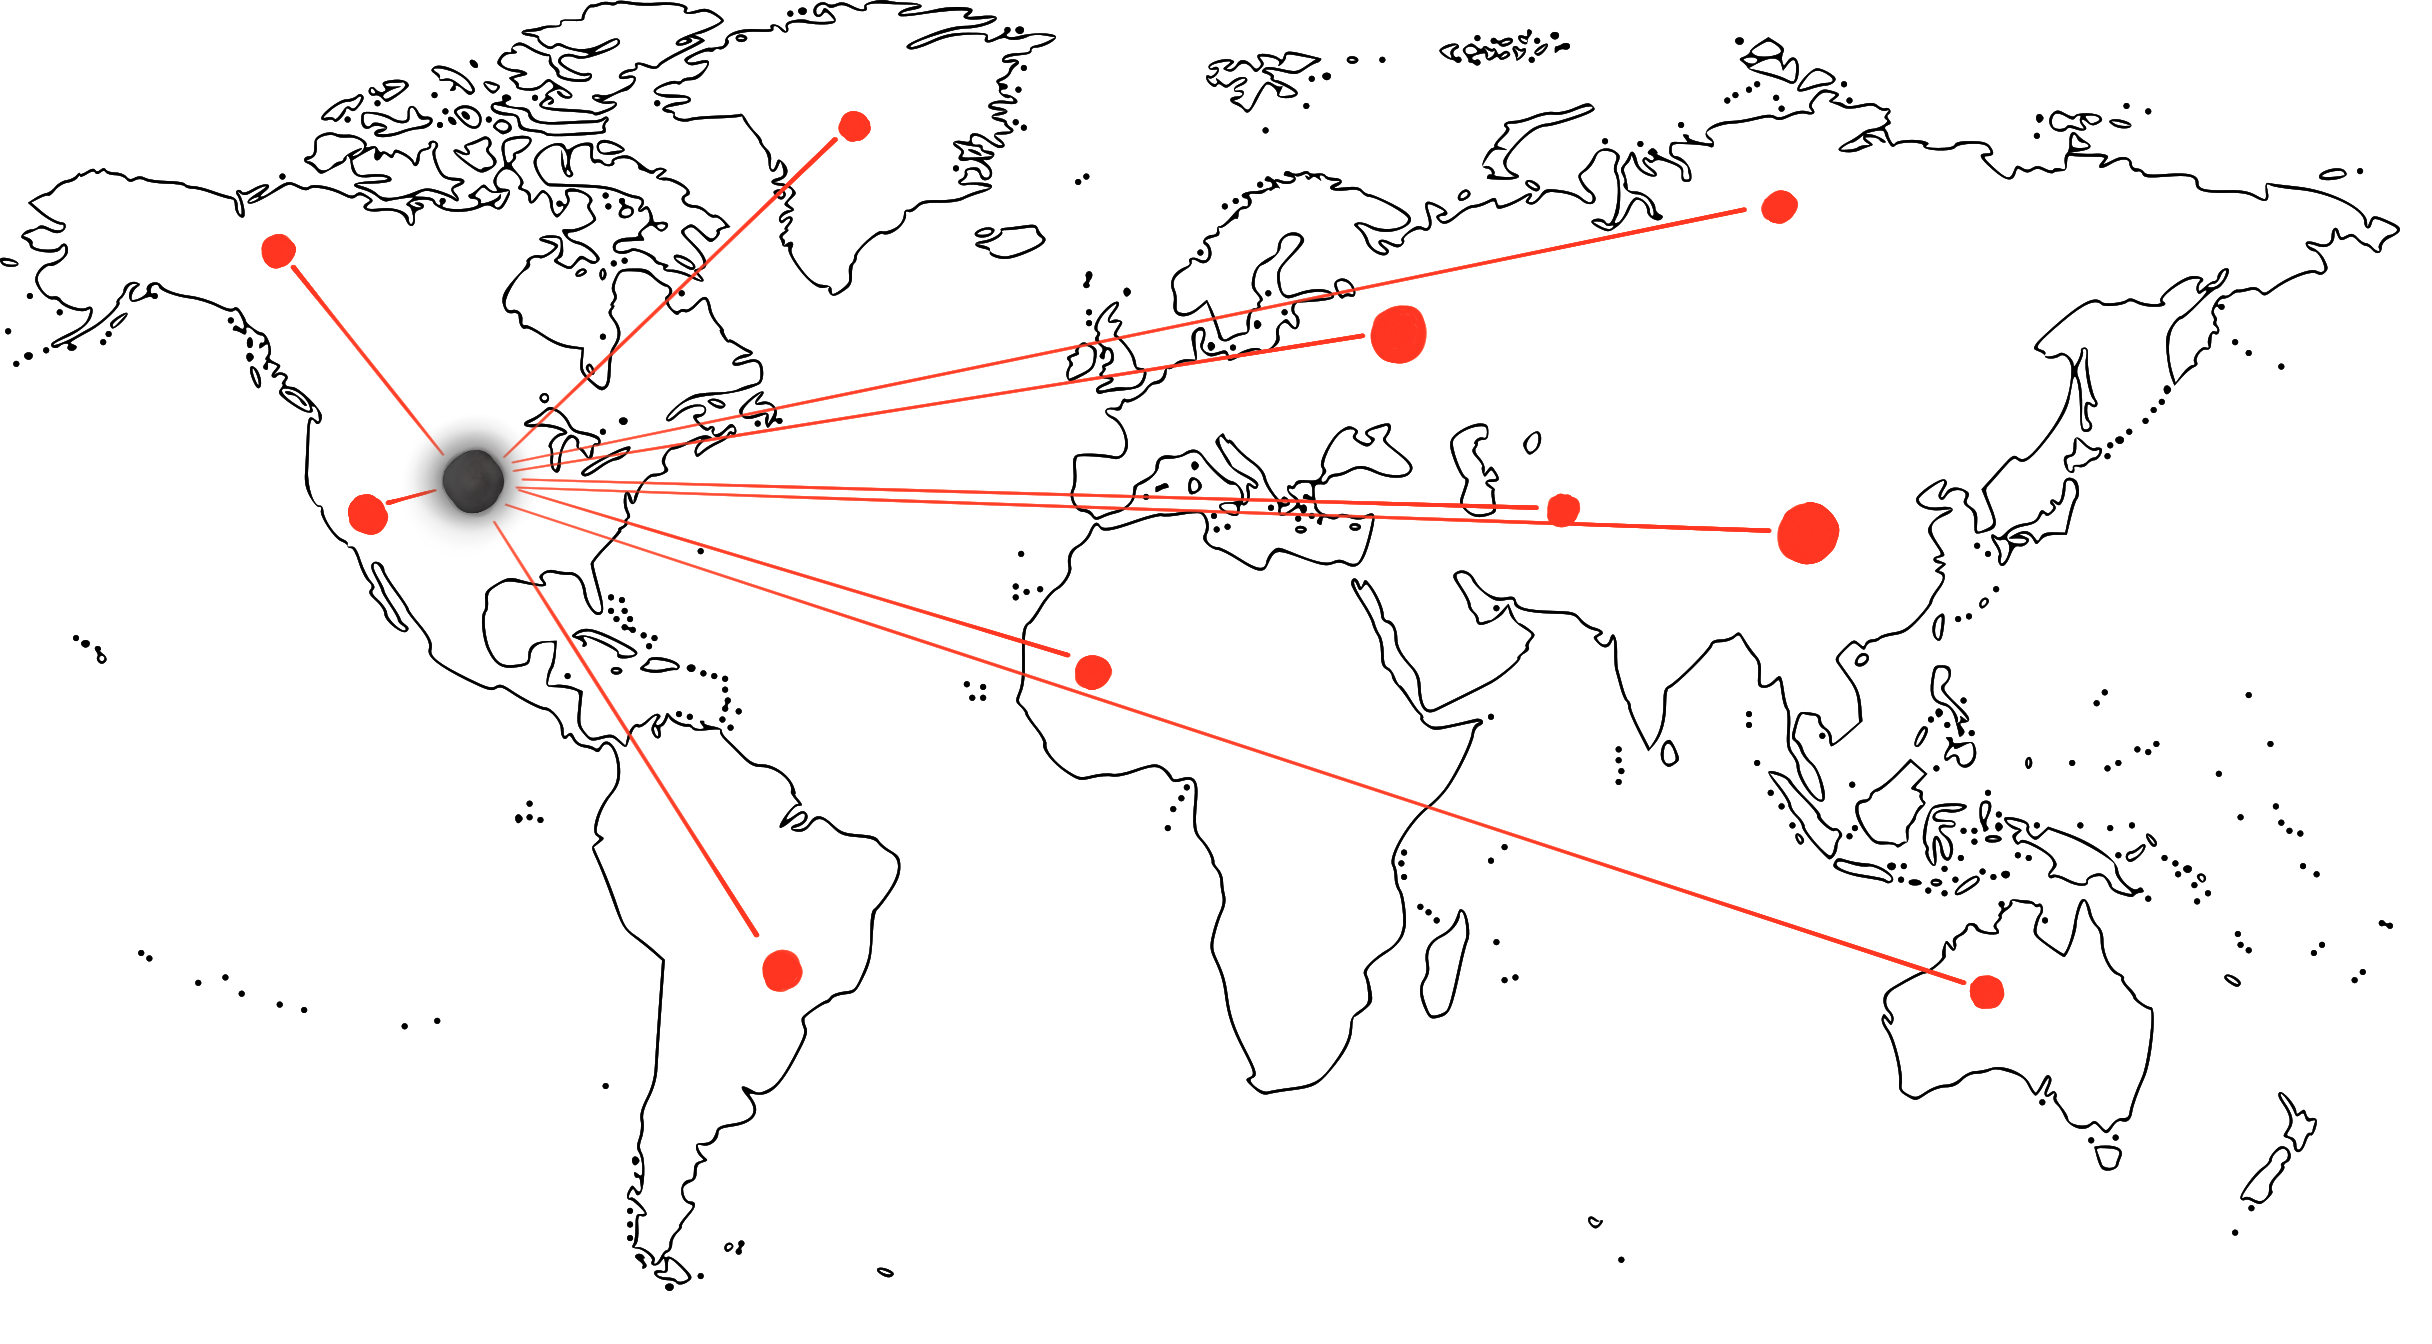
\includegraphics[width=\textwidth]{./images/world-map.png}
\end{frame}

\begin{frame}
	\frametitle{Wide-Area Big Data - WABD}
	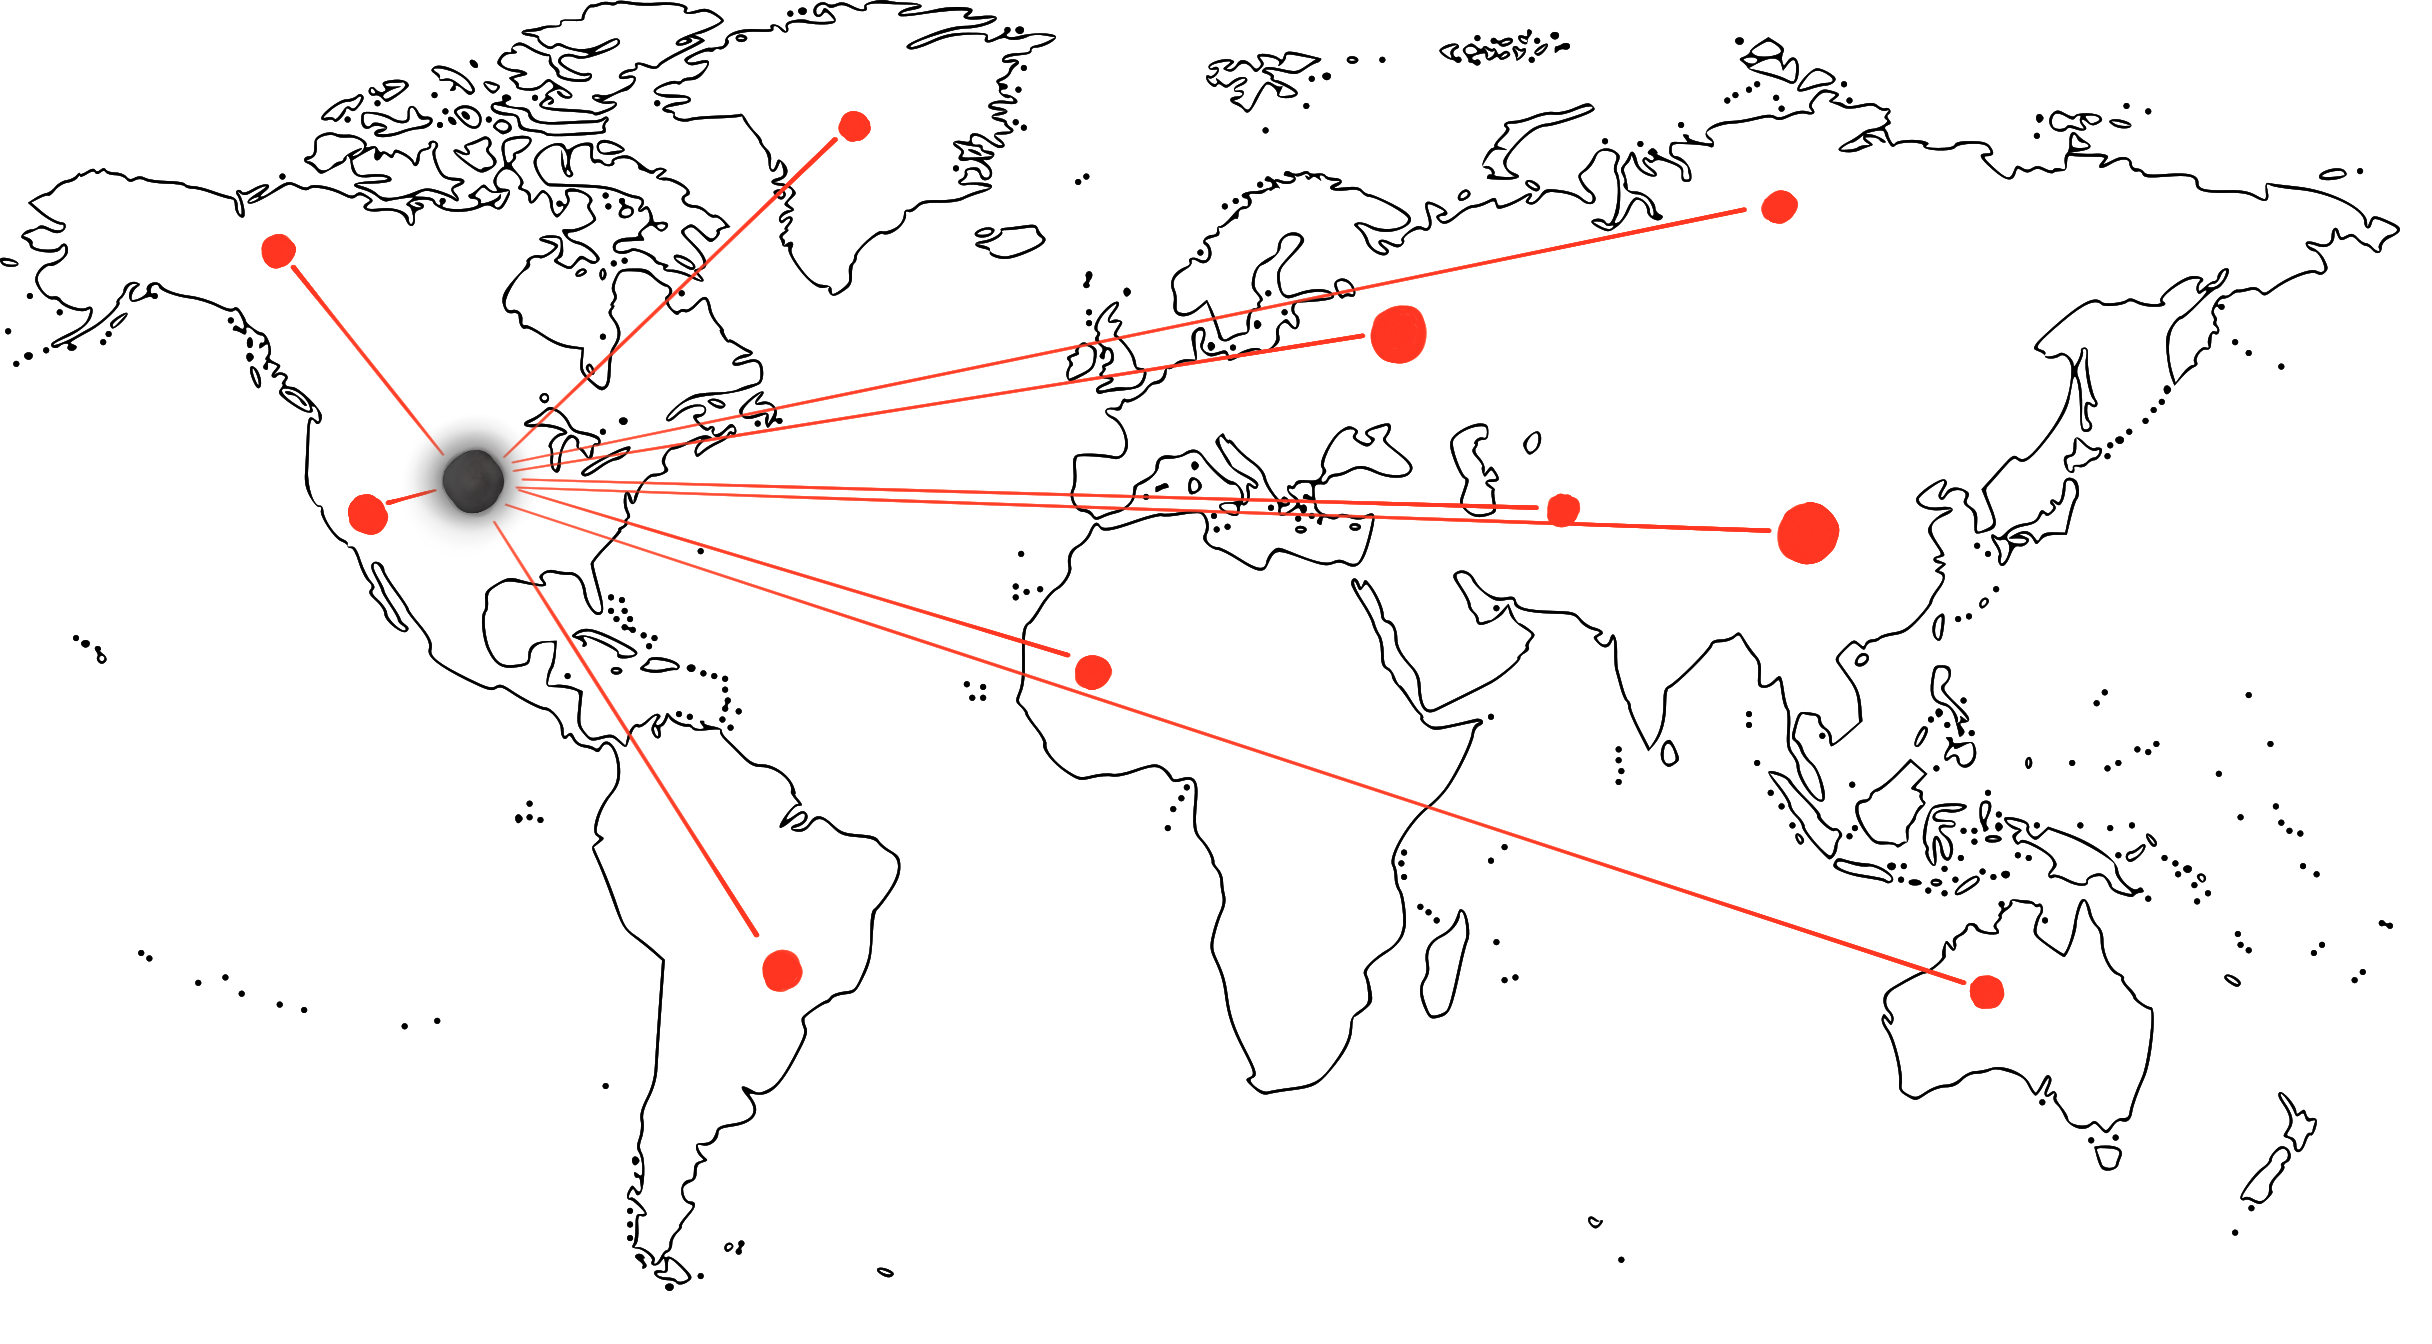
\includegraphics[width=\textwidth]{./images/world-map.png}
\end{frame}
%---------------------------------------------------------


\section{Second section}
%---------------------------------------------------------
\begin{frame}
	\frametitle{Sample frame title}

	In this slide, some important text will be
	\alert{highlighted} because it's important.
	Please, don't abuse it.

	\begin{block}{Remark}
		Sample text
	\end{block}

	\begin{alertblock}{Important theorem}
		Sample text in red box
	\end{alertblock}

	\begin{examples}
		Sample text in green box. The title of the block is ``Examples".
	\end{examples}
\end{frame}
%---------------------------------------------------------


%---------------------------------------------------------
%Two columns
\begin{frame}
	\frametitle{Two-column slide}

	\begin{columns}

		\column{0.5\textwidth}
		This is a text in first column.
		$$E=mc^2$$
		\begin{itemize}
			\item First item
			\item Second item
		\end{itemize}

		\column{0.5\textwidth}
		This text will be in the second column
		and on a second tought this is a nice looking
		layout in some cases.
	\end{columns}
\end{frame}
%---------------------------------------------------------


\end{document}
